\chapter{引言}
\label{cha:intro}

\section{课题研究背景}

BIOS(Basic Input Output System:基本输入输出系统)~\cite{1, 2},是一款能够被固化到计算机主板上的ROM(Read-Only Memory:只读存储器)芯片中的软件。其主要的功能,是为计算机提供最直接、最底层的硬件控制与设置,是连接计算机硬件体系和软件操作系统之间的桥梁。传统的BIOS由低级语言编写而成,采用十六位汇编作为基础构建其产品代码,以1MB为单位作为其固定的编址方式,采用寄存器参数作为其调用方式,采用静态链接作为其链接方式。因为BIOS是固化到ROM芯片中的,所以其也被称为Firmware(固件)。传统的BIOS发展至今其产品已相对成熟,但也暴露出些许缺点,例如:不便于引入新的技术对其功能进行扩展,开发和维护需要消耗较高的成本等一系列问题。

UEFI(Unified Extensible Firmware Interface:统一的可扩展的固件接口),是因特尔为了解决这些弊端所推出的新一代计算机固件接口标准,它对连接硬件体系和软件操作系统之间接口的标准进行了规定。~\cite{3} UEFI的提出更新了传统BIOS的技术,其采用高级语言和现代的软件工程方法来设计其程序结构,采用面向对象的思想作为指导来对产品的代码进行设计,各驱动、应用程序及其之间基于模块化的设计理念来进行规划,基于标准协议以实现模块和模块间的通信,这样做的优势显而易见。

伴随信息时代的来临以及不断进步和发展的软件技术水平,与传统的计算机工程的思想相比,作为确保软件质量最后也是最重要的一环的软件测试技术,在软件项目开发的进程中所处的重要地位越来越不容小视。在现代化的软件项目开发过程中,产品迭代开发的周期大大减少,需要开发人员对产品源文件频繁地进行修改和重构。这就需要软件测试的工作必须能够自动化的完成,以提高产品测试工作的质量与效率,否则无法对产品进行快速的开发。~\cite{4}

UEFI~\cite{5, 6}作为新一代的BIOS,其研发工作具有以下几个显著特点:1)开发周期长。2)庞大的API(Application Programming Interface:应用程序编程接口)库。3)不断扩展的API库。4)严格的质量要求。伴随UEFI BIOS开发过程中的软件测试工作,其需要针对产品的需求设计大量的Test Case(测试用例~\cite{7, 8})以验证产品的质量。为了完成这些预先设计好的测试任务,及时发现产品中潜在的缺陷,具备专业测试知识的QA(Quality Assurance:质量保障)需要耗费大量的时间和人力成本。然而UEFI BIOS产品的开发是一个长期的项目,其采用敏捷开发的模式,在产品研发过程中,每一个短暂的迭代周期都会对代码进行频繁的重构和修改,每一次扩展或者修改都会产生一个新版本的可执行产品,因此QA需要尽早对该版本的产品进行集成和测试,这样可以大大避免在项目后期产品进行集成时所出现的产品缺陷集中涌现的问题。然而随着项目开发过程的进行,QA的测试工作任务量会不断的提升和累加,他们不仅需要对每一个版本的产品进行迭代性和重复性的测试工作,同时还需要测试新版本产品添加的新的功能。如果采用手动测试机械重复的完成这些繁重的测试任务,毫无疑问是不明智也是低效的,这样做既不能保证测试工作的质量,也不能保证测试工作的正常进展。 因此,在有限的资源下,为了提高测试工作的效率、节省测试工作的成本、保证测试工作的进度和质量,采用持续集成的思想搭建一个自动化测试~\cite{9, 10, 11}系统用于完成从产品构建、产品部署、产品测试以及产品质量分析的UEFI BIOS测试工作就显得非常必要。

\section{国内外研究现状与发展动态}

\subsection{持续集成的国内外研究现状}
  
  在软件行业发展的初期软件开发人员基本上采用瀑布模型,软件开发中的集成~\cite{12}工作基本上都是在项目快要结束时进行的。此时将这些已经单独测试好并且能够正常独立运行的模块集成在一起后,系统整体却常常出现问题,并且很难找到问题的原因,这直接影响了软件的开发的周期和软件的质量。
  
  1999年,来自俄勒冈州大学的软件开发学的泰山北斗Kent Beck,首次提出了CI(Continuous Integration:持续集成)的理念。他认为,应该对产品项目的源代码经常进行集成工作,甚至于任何一个提交到版本控制库中的操作,都应该触发一次集成,这样做对于整个软件项目工程的顺利进行以及产品的高质量需求都有着极大的好处。为了体现敏捷开发的价值所在,也应该寻找合适的方法将软件的集成工作做到持续,找到合适的极致点以对产品进行频繁的集成。~\cite{13}为了满足不断提高的软件产品质量以及成倍增加的软件开发复杂度这一系列需求,作为敏捷开发发展历史上的一个重要的里程碑,CI这一概念的提出,成功的找到了一种合适的方法以保障软件产品项目的顺利有序进行。
  
  为了根据企业软件产品自身的特点,量身定制其各自的CI系统,大部分IT(Internet Technology:互联网技术)领域的成员依照CI的核心思想,开始逐渐发展CI的方法并且研发各自的CI工具,随之而来的产生了一大批持续集成的工具。和任何其他的软件产品一样,CI界较为常用的工具同样分为商业和开源两种不同的类型。开源产品的代表作之一CruiseControl,是最早出现的一款CI工具,它的出现使持续集成的研究迈入了一个新的时代,奠定了CI工具化的这一基点,同时为CI的发展做出了巨大的贡献。之后出现的Jenkins,是CI开源产品中的后起之秀,其利用Web实现了简洁的GUI(Graphical User Interface:图形用户界面),并且很容易进行使用,这是其最主要的特点~\cite{14}。与开源相对的是商用的CI工具,其中比较有代表性的是Bamboo 、TeamCity、QuickBuild和MavenHill这几款工具,具备相当高的市场占有率。
  
  作为开源CI工具的代表作,Jenkins这款软件于近几年来逐渐获得了市场上的大部分用户的青睐。Jenkins的安装配置较为简单,用户能够相对容易对其进行安装和配置,而且Jenkins具有插件支持、监控可视化等特点,其版本更新频率达到每周一次,更加值得一提的是,Jenkins在GitHub上具备强大的主导能力,这一系列的特点使得Jenkins在CI这一领域占据了大部分市场,并且遥遥领先于其他的CI工具。~\cite{15, 16}
  
  相对于国外,国内对于持续集成的研究与应用实践相对晚很多,很少有公司真正的把CI应用到其实际的产品项目开发中。然而近些年来,具有一定规模的大型互联网公司开始逐渐引入了CI的思想并且将其融入到了公司的实际项目中,这一点值得肯定。例如:百度作为中国互联网领域的巨头之一,从项目管理和需求管理等方面着手,开始引入敏捷开发的模式并且对其进行了实践,不断扩大的公司规模以及不断发展的公司业务要求需要其具备更高的软件项目开发速度和效率。于是百度在2010年正式采用了持续集成的策略,经过管理和开发人员的共同努力与不懈坚持,这一策略成功加以实施,并且给公司带来了很好的效益。

\subsection{测试工具的国内外研究现状}

  为了保障持续集成过程中软件的测试工作能够自动化的完成而不需要测试人员手动的去参与,针对特定软件产品的测试任务必须开发和使用特定的自动化测试工具,这是各个公司保障软件产品测试工作的质量和进度的最基本要求和发展方向。随着不断提升、进步和发展的软件测试水平以及技术,针对特定的测试任务,大量知名的互联网公司都开发并且发布了相应的测试工具,以用于自动化的对软件产品进行验证。以下简要介绍三款工具:
  
  \begin{itemize}
	\item IBM Rational Robot
	
	  作为Rational系列软件产品的代表之一,IBM Rational Robot~\cite{17}能够提供自动化的测试手段,用于重复性和机械性的执行软件测试任务。利用该款工具,大大方便了为了验证产品质量而执行测试用例工作的QA的效率,节省了他们的时间成本。针对Java、Web、.NET以及其他基于GUI的软件产品,QA能够利用其在无人值守的情况下自动化的执行产品对应的功能性回归测试任务~\cite{18}。
	
	\item HP QuickTest professional
	
	  HP QuickTest professional~\cite{19}是目前市场上最常用的软件测试工具之一。其出现使得对产品的功能测试和回归测试变成了自动化的测试~\cite{20, 21}。用户预先在屏幕上进行相应的测试操作流程,QTP能够对其进行录制并且自动的生成测试用例和测试脚本。该工具的主要优点是适用性好、操作简单、脚本通俗易懂,即便是没有代码基础和经验的QA也能够利用其进行脚本的录制与调试操作。但是QTP具有一个较为明显的缺点:其基于关键字的框架在灵活性方面效果较差~\cite{22, 23}。
	  
	\item HP Mercury LoadRunner

	  HP Mercury LoadRunner~\cite{24}作为负载测试工具主要用于对产品进行性能测试,以便于开发人员优化系统的性能、预测系统的行为。这是基于模拟的手段,以实现真实情况下海量用户在同一时间对产品执行频繁操作的情景,从而对产品的性能进行实时的监测,以发现产品存在性能缺陷,从而对整个产品的系统架构进行优化。利用此方式大大减少了软件的测试时间消耗~\cite{25, 26}、促进和优化了系统的性能并且缩短了产品版本的研发时间和发布周期。
  \end{itemize}
  
  从中可以看出,自动化测试工具在国外软件测试的相关领域中,已占据了重要的地位。其主要代表如表~\ref{tab:常用的测试工具}所示:
  
  	\begin{table}[H]
		\centering
		\caption{常用的测试工具~\cite{27}}
		\label{tab:常用的测试工具}
		\begin{center}
		\begin{tabular}{|l|l|l|} 
		\hline
		适用于的测试种类 & 测试工具的名称 & 生产厂家 \\ \hline
		性能测试 & JMeter & Apache \\ \hline
		性能测试 & LoadRunner & HP \\ \hline
		功能测试 & Selenium & ThoughtWorks \\ \hline
		功能测试 & Rational Function Tester & IBM \\ \hline
		功能测试 & QTP & HP \\ \hline
		功能测试 & WinRunner & HP \\ \hline
		单元测试(Java) & TestNG & 开源(Apache) \\ \hline
		单元测试(Java) & Junit & 开源(Unix) \\ \hline
		\end{tabular}
		\end{center}
	\end{table}
  
  在国内,自动化软件测试仍处于起步阶段,知名的测试工具比较少。虽然与国外相比确实存在一定的差距,但是伴随着最近几年不断扩大规模的某些个产品厂家的出现,他们都参考并引入了大量国外的自动化测试工具,以在产品开发过程中利用其自动化的执行软件测试任务。针对已有测试工具并不能满足需求的这一问题,许多已具备相当规模的互联网公司甚至针对自身产品的特点开发了特有的测试工具,这一进步值得肯定。但是由于较高的维护成本和快速变化的功能需求,大多数的测试工具仍然仅仅使用了自动化测试的理念而没有利用好自动化测试的优势。
  
\section{本文的选题依据}

  首先UEFI BIOS测试工作有着成百上千的测试用例,需要耗费QA大量的时间去完成,针对产品的传统手动测试,既无法保障测试工作的高质量完成,也无法保障测试工作的快速进行,因而需要使用测试工具自动化的对其进行测试,以降低人力和时间成本。与传统的软件测试相比,UEFI BIOS的测试工作与之有着许多不一样的地方:第一,现有大多数的测试工具都是运行在OS(Operating System:操作系统)环境中的,然而UEFI BIOS并不是运行在该环境之中,而是运行在OS环境之下,因此QA需要对未加载操作系统的测试机上,对UEFI BIOS进行测试,因而无法利用现有的测试工具,完成这一测试任务;第二,UEFI BIOS的运行需要一些硬件进行参与,然而涉及到硬件的参与,对于UEFI BIOS的系统稳定性和缺陷率便相对较高,例如,Recovery Mode、 Clear CMOS(Complementary Metal Oxide Semiconductor:互补金属氧化物半导体)等计算机主板上的跳线、DC(Direct Current:直流电)和AC(Alternating Current:交流电)的开关等等。针对上述几个问题,现有的所有自动化软件测试工具都没有办法解决。因此,我们首先要解决的问题便是设计和实现一套稳定可靠、性能良好的测试工具,用于利用其自动化的完成对应的UEFI BIOS测试工作。
  
  其次,作为长期项目的UEFI BIOS产品研发过程,在其敏捷开发的过程中,在每一个短暂的迭代周期中,都会相应的产生一个新版本的可执行产品,这需要开发人员与测试人员密切协作,QA需要尽早对产品进行集成和测试以避免产品在开发收尾阶段产品缺陷的集中涌现,如图~\ref{fig:迭代式开发中的开发人员与测试人员的合作}所示。并且随着开发的进行,测试任务工作量会逐步累加,为了提高测试效率、节省测试成本、保证测试工作的进度以及保证测试工作的质量,基于持续集成的思想搭建一个自动化测试系统用于完成从产品构建、产品部署、产品测试以及产品质量分析的UEFI BIOS集成测试工作就显得非常必要。
  
	\begin{figure}[H] % use float package if you want it here
		\centering
		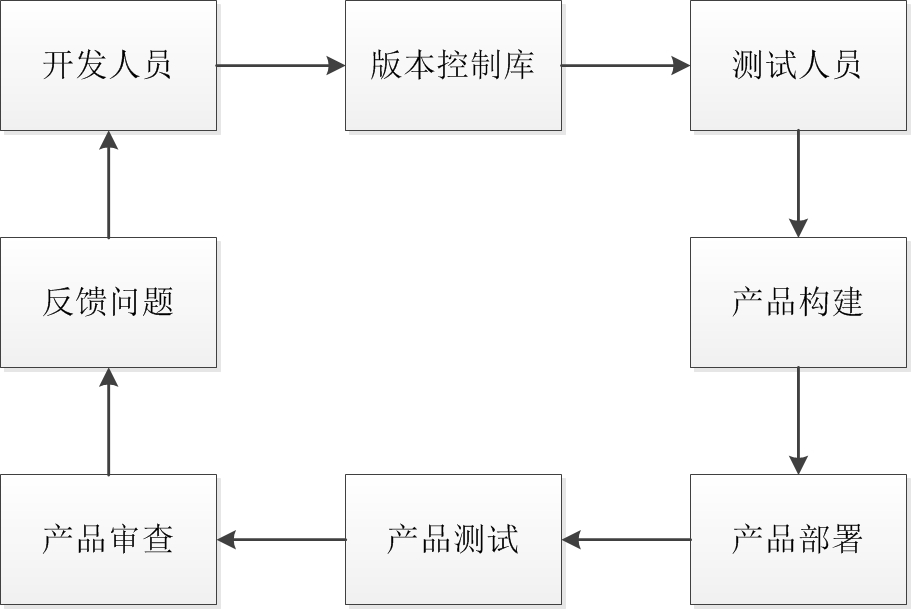
\includegraphics[height=7cm]{chart1/迭代式开发中的开发人员与测试人员的合作}
		\caption{迭代式开发过程中开发人员与测试人员之间的协作}
		\label{fig:迭代式开发中的开发人员与测试人员的合作}
	\end{figure}
  
\section{本文主要研究内容}

  \begin{itemize}
	\item 针对涉及到硬件的软件测试以及非OS下的软件测试,我们在基于EFI$\backslash$UEFI标准下,结合BIOS软件测试的实际需求,开发了一套测试工具SCT(Self-Certification Test:自我认证测试)~\cite{28, 29}用于对产品进行功能性测试,以验证产品中各种功能是否存在缺陷,对测试结果进行分析和总结以生成相应的报告。该测试工具在UEFI BIOS的Shell环境中~\cite{30, 31}运行,支持白盒、黑盒等不同类型的测试。总的来说,SCT具有以下几个特点:
	  \begin{itemize}
		\item 能够自动化的执行用例,对UEFI BIOS进行测试和验证,及时发现其中可能存在的问题和缺陷,以便于提高软件的质量。
		\item 能够执行多种测试类型,例如白盒、黑盒等不同类型测试。
		\item 能够分析每一个用例的执行结果,并且对全部用例的测试结果进行总结,生成相应的测试报告。
		\item 当工具运行发生意外中断时,能够记录中断的位置,在工具再次执行时从该位置继续执行之后的用例,而不需要对已执行的用例进行重复的测试。
		\item 具备良好的GUI,能够方便QA便捷的利用测试工具对测试用例进行管理和设置,控制需要执行的用例。
	  \end{itemize}
	\item 为了在有限的资源下,提高测试工作的效率、节省测试工作的成本、保证测试工作的进度和质量。我们搭建了一套可以无人值守的持续集成测试系统用于UEFI BIOS开发过程中每日的迭代性集成测试。该系统基于持续集成的思想,能够自动化的实现从产品构建、产品部署、利用SCT对其进行功能性测试、解析测试结果生成测试报告并且向开发人员反馈该系统测试出的产品缺陷这一系列复杂的测试流程,是持续集成理论的又一次成功实践。该系统总的来说具有以下几个特点:
	  \begin{itemize}
		\item 系统中的任一环节都是自动完成的,有利于减少测试任务中的重复过程所耗费的时间和人力成本。
		\item 系统能够尽早、及时的发现软件不能够构建或者存在产品缺陷的问题,使随时(快速、可靠、低风险)发布功能正常的软件成为了可能。
		\item 系统尽早、尽快进行集成,有助于尽早发现产品中存在的缺陷,避免最终产品集成中出现Bug(缺陷)大量涌现的情况,这样容易及时定位和修正Bug,提高产品开发的质量与效率。
		\item 保证了敏捷开发过程中软件项目的进度和质量。
	  \end{itemize}
  \end{itemize}

\section{论文的组织}
	
	第一章引言,介绍了课题的研究背景和现状,说明了选题依据和来源,简要的介绍了本文的工作,给出了本文的主要研究点和组织。
	
	第二章主要介绍了集成测试与持续集成测试的思想,针对现有CI引擎工具不满足UEFI BIOS的需求这一问题,提出了设计需求,为UEFI BIOS自动化测试系统的设计和实现做好了理论铺垫。
	
	第三章主要分析对比了现有的各种测试工具,针对其不适合非OS下的UEFI BIOS测试任务这一问题,设计并且实现了一款新的测试工具SCT专门用于UEFI BIOS的功能性测试,而产品测试的工作能够利用该工具在无人值守的情况下自动化的完成,正是持续集成测试系统中重要的组成部分。
	
	第四章主要介绍X-64架构(特定的CPU架构)的Denlow平台持续集成测试系统的设计与实现,并且展示了已经成功应用到Denlow-X64的实际开发项目中的系统实验结果。
	
	第五章主要介绍IA-32架构(特定的CPU架构)的Nt32平台持续集成测试系统的设计与实现,并且展示了已经成功应用到Nt32-IA32的实际开发项目中的系统实验结果。
	
	第六章对本文的工作的优缺点进行了归纳,并且提出了进一步的研究目标。
	
\section{本章小结}
  
    本章第一小节主要介绍了BIOS、UEFI、软件测试与UEFI BIOS软件测试的特点等这些课题的背景情况。
	
	本章第二小节主要介绍了测试工具和持续集成的研究情况。
	
	本章第三小节主要说明了本文的选题依据和来源,阐明了本文所具有的理论价值和实际应用价值。
	
	本章的第四小节说明了本文的主要研究内容。
	
	本章的第五小结说明了本文的组织情况。

	